\section{Spiegelladung}
\begin{figure}
 \centering
 \includegraphics{media/spiegelladung.pdf}
\end{figure}
\begin{figure}
    \centering
    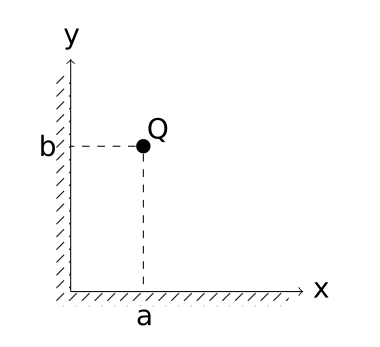
\includegraphics{media/Skizze.png}
   \end{figure}
\pagebreak

\section{Aufgaben}
\subsection{Aufgabe: Kraftfeld}
Gegeben sei ein Kraftfeld
\begin{equation}
    \vec{F} (\vec{r}) = 
\begin{pmatrix*}[c]
a(3x − y) \\
b(2y − x)
\end{pmatrix*}
\end{equation}
mit a, b = const.
Ein punktförmiges Teilchen befinde sich in dem Kraftfeld $\vec{F} (\vec{r})$. Berechnen Sie die Arbeit, die
beim Verschieben entlang der folgenden Wege geleistet wird:
 
\begin{equation*}
    \text{(a)}\; \vec{r}_1 (t) = 
\begin{pmatrix*}[c]
t \\
t
\end{pmatrix*}
\text{mit}\; t \in [0, 2]
\end{equation*}

\begin{equation*}
    \text{(b)}\; \vec{r}_2 (t) = 
\begin{pmatrix*}[c]
t \\
\frac{t}{2}^2
\end{pmatrix*}
\text{mit}\; t \in [0, 2]
\end{equation*}

\begin{equation*}
    \text{(c)}\; \vec{r}_3 (t) = 
\begin{pmatrix*}[c]
    2c \cos(t) \\
    3c \sin(t)
\end{pmatrix*}
\text{mit}\; t \in [0, 2\pi]
\end{equation*}

\subsection{Aufgabe: Delta-Distribution}
Berechnen Sie 

a) die Ableitung
\begin{equation*}
    \int_{a}^{b} f(x) \delta'(x)\, dx
\end{equation*}

b) eine Skalierung und Verschiebung
\begin{equation*}
    \int_{a}^{b} f(x) \delta(cx- d)\, dx
\end{equation*}
c) und die Verkettung mit g
\begin{equation*}
    \int_{a}^{b} f(x) \delta(g(x))\, dx
\end{equation*}


von $\delta.$ 

\subsection{Aufgabe: Dielektrische Flüssigkeit im Zylinderkondensator}

Ein Zylinderkondensator bestehe aus zwei konzentrischen Röhren der Länge $L = 1 \si{\meter}$, wobei der
Abstand $d = 1 \si{\milli\meter}$ zwischen den Röhren als klein gegen ihre Radien angenommen werden soll.
Nachdem der Kondensator mit einer Gleichspannungsquelle (U = 200 V) aufgeladen wurde, wird
das untere Ende des Kondensators in destilliertes Wasser knapp eingetaucht (Dichte ρ = 1 g/cm 3 ,
Dielektrizitätszahl ε = 81; Leitfähigkeit, kapillare Kräfte und Eintauchtiefe sind zu vernachlässi-
gen). Das Wasser steigt im Kondensator, wobei die zusätzliche Energie (potenzielle Energie des
Wassers und Feldenergie) von der Spannungsquelle geliefert wird.
Berechnen Sie die Höhe h der Wassersäule, die sich nach dem Einschwingen einstellt, indem Sie die
wirkenden Kräfte betrachten.

\subsection{Aufgabe: Satz von Gauß}
\begin{equation}
\vec{v} (x, y) =
\begin{pmatrix*}[c]
    x + e^{−y^2} \\
    y + e^{−x^4}
\end{pmatrix*}
\end{equation}
 Berechnen Sie den Fluss durch das Einheitsquadrat mit Hilfe des Satzes von Gauß.
